\documentclass[tikz]{standalone}
\usepackage{tikz}

\begin{document}    
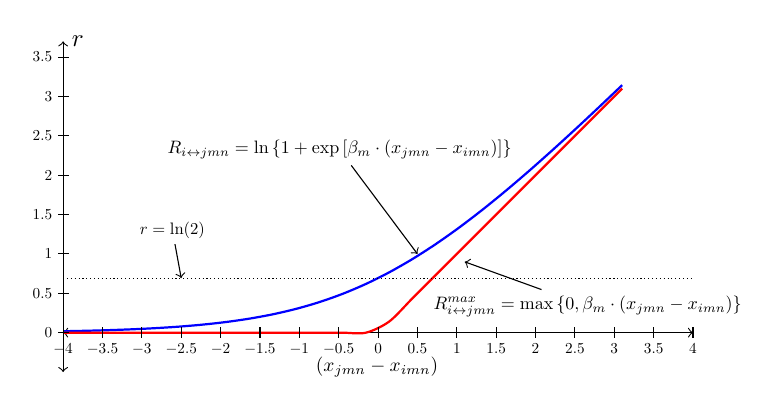
\begin{tikzpicture}
 \usetikzlibrary{positioning}
 \node (center) {};
 
 
 %Coordinates
 \coordinate (maxRRMcoordinate) at (1.1,0.9);
 \coordinate (RRMcoordinate) at (0.5,1);
 \coordinate (ln2coordinate) at (-2.5,{ln(2)});
 
 
 %Names
 \node (maxRRM) [scale=0.65,above right=0cm and .5cm of center  ] {$R^{max}_{i\leftrightarrow jmn} = \max\left\{0,\beta_{m}\cdot\left(x_{jmn} - x_{imn}\right)\right\}$};
 
 \node (RRM) [scale=0.65,  above left =2cm and -1.9cm   of center] { $R_{i\leftrightarrow jmn}=\ln\left\{1 + \exp\left[\beta_{m}\cdot\left(x_{jmn} - x_{imn}\right)\right]\right\}$};
 
 \node (ln2name) [scale=0.6,  above left =1cm and 2cm   of center] { $r=\ln(2)$};
 
 
 %Axis
   \draw[<->] (-4, 0) -- (4, 0) node[scale=0.7, below right = 0.1cm and -1cm of center] {$(x_{jmn} - x_{imn})$};
  \draw[<->] (-4, -0.5) -- (-4, 3.7) node[right,scale=0.9] {$r$};
  
 %Functions 
  \draw[scale=1, domain=-4:3.1, smooth ,variable=\x, blue,thick ] plot  ({\x}, {ln(1+exp(\x))});
  \draw[scale=1, domain=-4:3.1, smooth, variable=\x, red,thick] plot ({\x}, {max(0,\x)});
  \draw[scale=1, domain=-4:4, densely dotted, variable=\x, black] plot ({\x}, {ln(2)});

 \foreach \x/\xtext in {0,0.5,1,1.5,2,2.5,3,3.5,4}
\draw[shift={(\x,0)}] (0pt,2pt) -- (0pt,-2pt) node[scale=0.55,below] {$\xtext$};

 \foreach \x/\xtext in {0.5,1,1.5,2,2.5,3,3.5,4}
\draw[shift={(-\x,0)}] (0pt,2pt) -- (0pt,-2pt) node[scale=0.55,below] {$-\xtext$};

  \foreach \y/\ytext in {0,0.5,1,1.5,2,2.5,3,3.5}
  \draw[shift={(-4,\y)}] (2pt,0pt) -- (-2pt,0pt) node[scale=0.55,left] {$\ytext$};
  %Labels of functions

  \draw[->] (maxRRM) -- (maxRRMcoordinate);
  \draw[->] (RRM) -- (RRMcoordinate);
   \draw[->] (ln2name) -- (ln2coordinate);
  
\end{tikzpicture}
\end{document}


